%\documentclass[fleqn, letterpaper]{amsart}
\documentclass[fleqn, letterpaper]{tufte-handout}
\usepackage{times}
\usepackage{amsmath}
\usepackage{graphicx}
\usepackage{booktabs}
\usepackage{multirow}
%\usepackage[left=1in]{geometry}

\newcommand{\R}{\mathcal{R}}
\newcommand{\E}{\text{E}}
\newcommand{\p}{p_{XY}}
\renewcommand{\arraystretch}{1.5}

\title{Problem Set 3 --- ENCE689E Spring 2014}
\author{David Prentiss}

\begin{document}
\maketitle

\section{1. Monte Carlo Methods}
\subsection{(a), (b)}
\newpage
\subsection{(c), (d)}
See Figure \ref{rand} and the following code:
\small
\begin{verbatim}
syms x;
pdf = sym(exp(-x));    % define exponential density function
cdf = int(pdf, 0, x);  % integrate pdf to find cdf
F = finverse(cdf);     % calculate inverse of cdf
rng(1);                % set random seed for reproducible results

plotNum = 0;
% calculate and plot ensembles generated with rand
for n = [10 100 1000 10000]
    bins = 0:0.1:10;
    r = rand(n, 1);                % generate random probabilties
    mc = subs(F, 'x', r);          % calculate z values
    [count, loc] = hist(mc, bins);
    
    % plot figure 1
    figure(1)
    plotNum = plotNum + 1;
    subplot(2, 2, plotNum)
    bar(loc, count/n*10, 'EdgeColor', 'none', 'BarWidth', 1); hold on;
    d = 0:0.01:6;
    plot(d, exp(-d));
    axis([0, 6, 0, 1]);
    title(['exp(-x), n=', num2str(n)]);
    set(findall(gcf,'type','text'),'fontSize',18);
    set(gca,'fontSize',18);
end

plotNum = 0;
% calculate and plot ensembles generated with exprnd
for n = [10 100 1000 10000]
    bins = 0:0.1:10;
    r = exprnd(1, n, 1);           % generate random probabilties
    mc = subs(F, 'x', r);          % calculate z values
    [count, loc] = hist(mc, bins);
    
    % plot figure 2
    figure(2)
    plotNum = plotNum + 1;
    subplot(2, 2, plotNum)
    bar(loc, count/n*10, 'EdgeColor', 'none', 'BarWidth', 1); hold on;
    d = 0:0.01:6;
    plot(d, exp(-d));
    axis([0, 6, 0, 1]);
    title(['exp(-x), n=', num2str(n)]);
    set(findall(gcf,'type','text'),'fontSize',18);
    set(gca,'fontSize',18);
\end{verbatim}
\subsection{(e)}

\begin{figure*}
    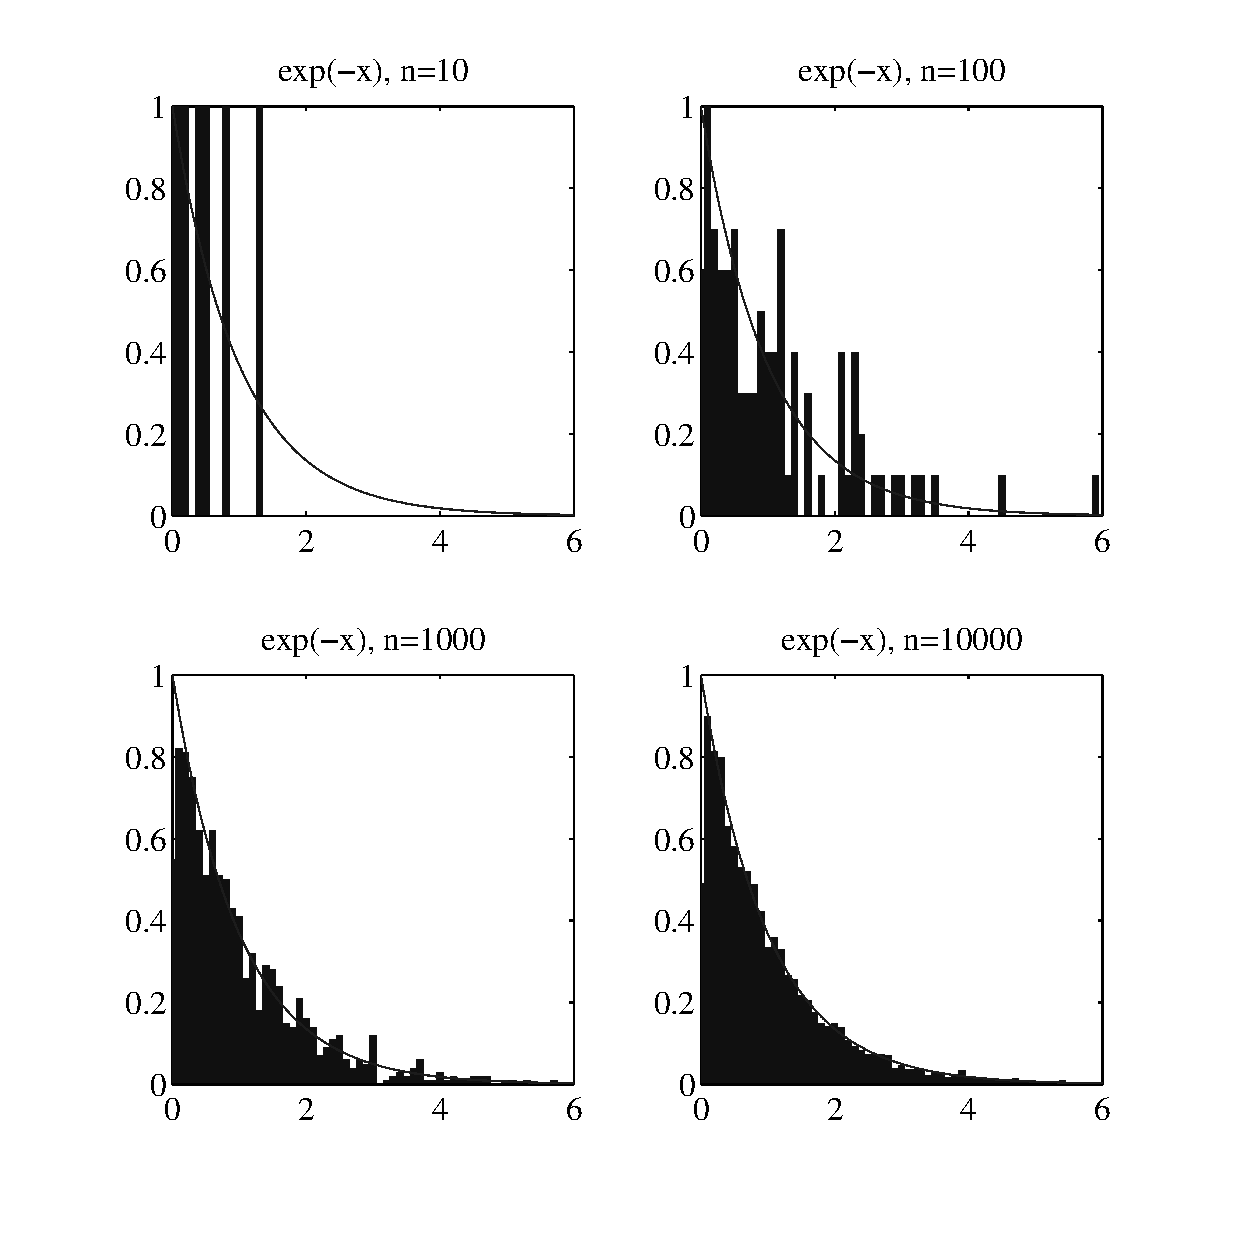
\includegraphics[width=0.8\textwidth]{problem1}
    \caption{Ensebles generated with the inverse cumulative distribution function}
    \label{rand}
\end{figure*}
\begin{figure*}
    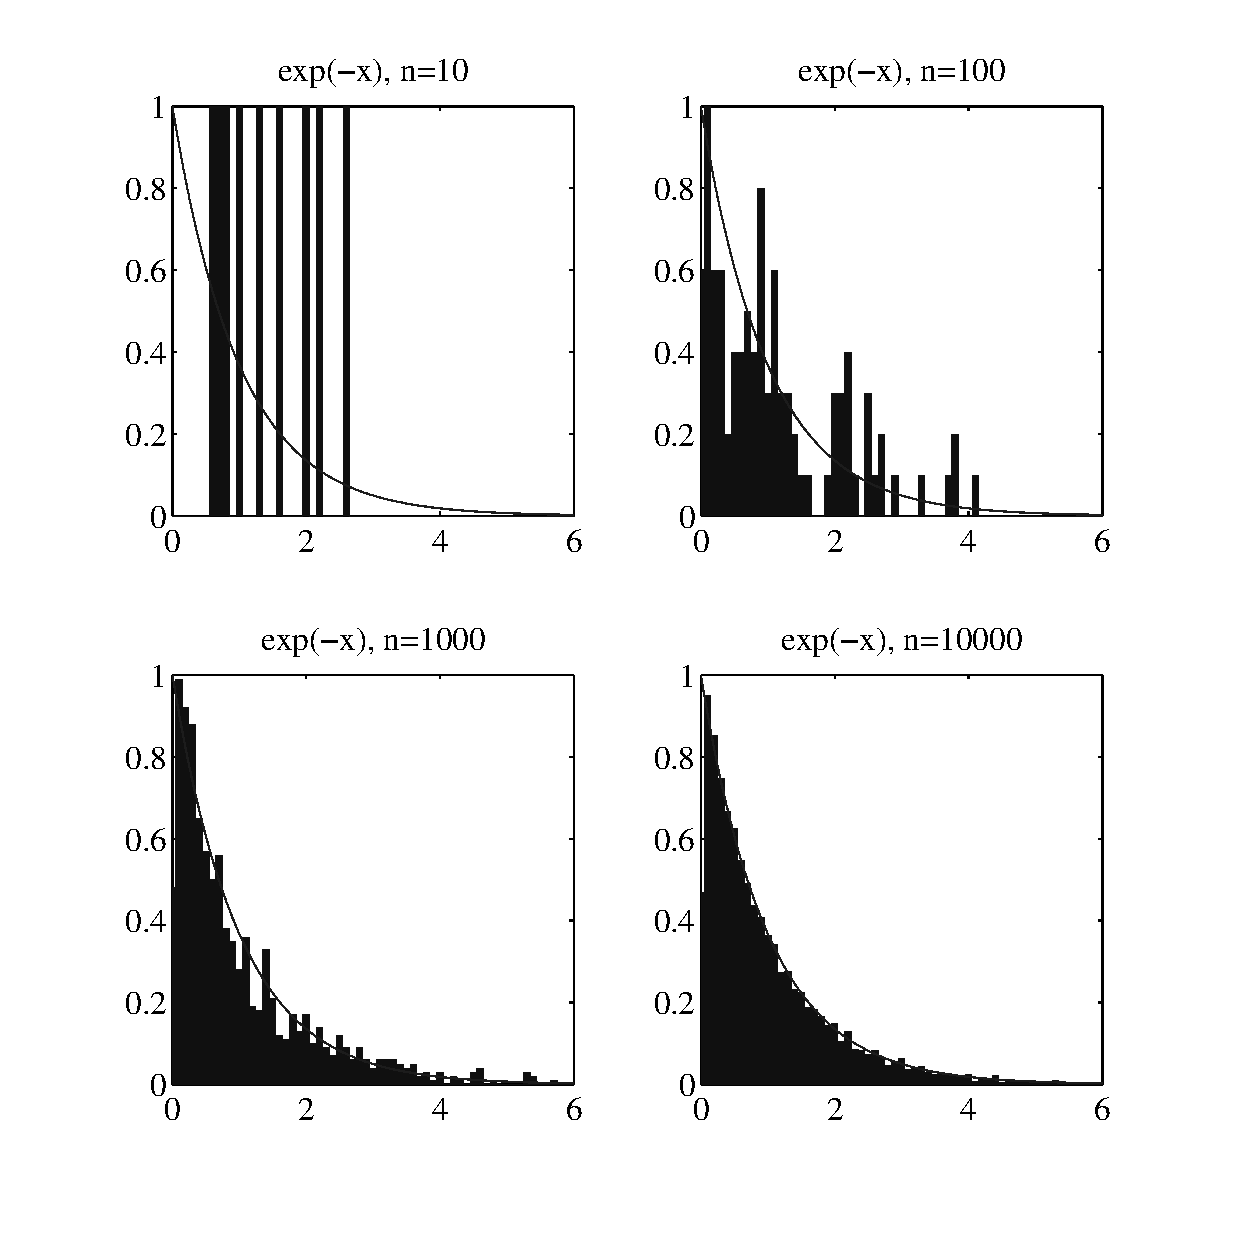
\includegraphics[width=0.8\textwidth]{problem1e}
    \caption{Ensebles generated with the MATLAB {\ttfamily exprnd} function}
    \label{exprnd}
\end{figure*}
\end{document}